\documentclass[Space3_Assign2]{subfile}

\begin{document}

\begin{figure}
\centering
\caption{GPS 24 hr simulation with dt = 100 in ECI frame}
\label{Q1AECI}
\includegraphics[width = \linewidth]{./Q1AECI.jpg}
\end{figure}

\begin{figure}
\centering
\caption{GPS 24 hr simulation with dt = 100 in ECI frame}
\label{Q1AECIside}
\includegraphics[width = \linewidth]{./Q1AECI_side.jpg}
\end{figure}

\begin{figure}
\centering
\caption{GPS 24 hr simulation with dt = 100 in ECEF frame}
\label{Q1AECEF}
\includegraphics[width = \linewidth]{./Q1AECEF.jpg}
\end{figure}

\begin{figure}
\centering
\caption{GPS 24 hr simulation with dt = 100 in ECEF frame}
\label{Q1AECEFside}
\includegraphics[width = \linewidth]{./Q1AECEF_side.jpg}
\end{figure}

\begin{figure}
\centering
\caption{GPS 24 hr simulation with dt = 100 Ground Trace}
\label{Q1AGT}
\includegraphics[width = \linewidth]{./Q1AGT.jpg}
\end{figure}

\begin{figure}
\centering
\caption{UAV trace in NED coordinates from the ground station at [Lat 34.76\Deg,Long: 150.03\Deg E, Alt: 680m]}
\label{Q1BF1LG}
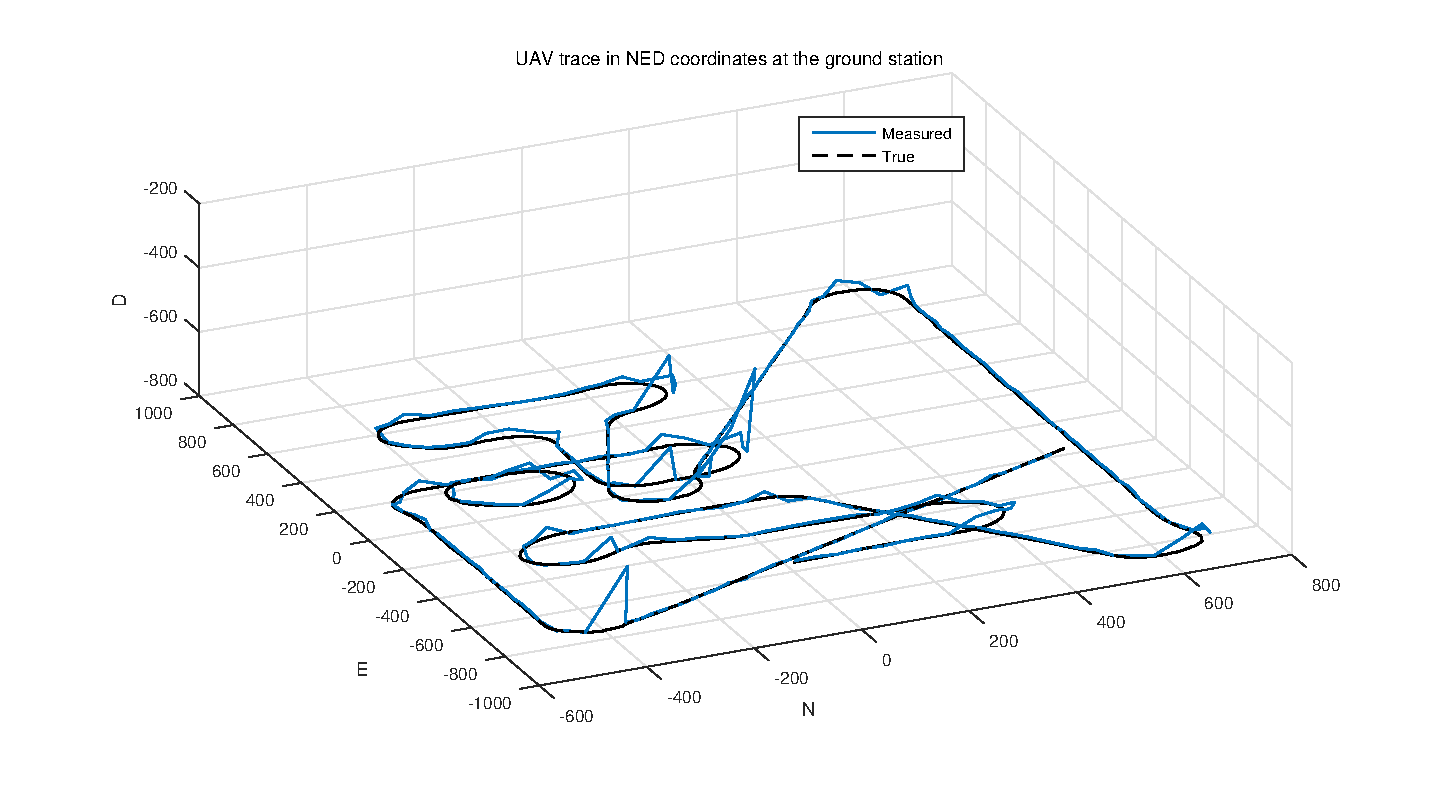
\includegraphics[width = \linewidth]{./Q1B_F1_LG.eps}
\end{figure}

\begin{figure}
\centering
\caption{UAV polar trace of azimuth and elevation and location of observed satellites from ground station at [Lat 34.76\Deg,Long: 150.03\Deg E, Alt: 680m]}
\label{Q1B_polartrack}
\includegraphics[width = \linewidth]{./Q1B_polartrack.eps}
\end{figure}


\end{document}